\pdfoutput=1
% main_v4 (2026-11-29 rewrite): the hackathon template's order, plain language, every short name explained where it
% first appears. Same results and numbers as before; every number resolves to a file named here or in
% paper/EVIDENCE_LEDGER_V4.md. The previous text is in main_v4_prerewrite.tex.bak (local) and in git history.
\documentclass[11pt]{article}
\usepackage{emnlp2023}
\usepackage{times}
\usepackage{latexsym}
\usepackage[T1]{fontenc}
\usepackage[utf8]{inputenc}
\usepackage{microtype}
\usepackage{booktabs}
\usepackage{url}
\def\UrlBreaks{\do\/\do\_\do\.\do\:\do\-}
\usepackage{graphicx}
\usepackage{xcolor}
\usepackage{amsmath,amssymb,amsthm}
\newtheorem{theorem}{Theorem}
\newtheorem{proposition}{Proposition}
\newtheorem{corollary}{Corollary}
\newcommand{\sgn}{\operatorname{sign}}
\newcommand{\judgebox}[1]{\par\smallskip\noindent\fcolorbox{black!60}{black!4}{\parbox{\dimexpr\columnwidth-2\fboxsep-2\fboxrule}{\small #1}}\par\smallskip}
\raggedbottom
\setlength{\textfloatsep}{8pt plus 2pt minus 2pt}\setlength{\floatsep}{8pt plus 2pt minus 2pt}\setlength{\dbltextfloatsep}{8pt plus 2pt minus 2pt}

\title{The Hidden World in the Group:\\How GRPO Mislearns Costly Verification in Agentic RL}

\author{Atharv \\
  Lexsi Labs hackathon 2026 \\
  \texttt{github.com/atharvgaur1845/actionproof-v2}}

\begin{document}
\maketitle

\begin{abstract}
AI agents that act through tools often get a reply such as ``ok'' that does not prove what happened. A careful agent
can check, for example by reading the payment record back, but checking costs time. We study what a popular training
method, group-relative policy optimisation (GRPO), teaches an agent about when to check. GRPO samples a group of
attempts at the same task and scores each attempt relative to the others. In a tool environment, all attempts at one
task usually face the same hidden situation: the same database and the same silent fault. We show that GRPO's
scoring then cancels out how much each hidden situation matters. What is left is a vote: the agent learns to check if
most hidden situations favour checking, however rare and expensive the others are. We prove when this happens and
when it does not. We registered our predictions before testing them. On 731 held-out analytical test cases, the
theory predicts GRPO's learned decision in all 721 cases that have a clear answer; one registered hypothesis failed
and one could not be tested, and we report both. We then trained a 3.35-billion-parameter Cohere tool agent (Tiny Aya
Global) five times with each method. With standard GRPO the agent never learned to check, in all five runs; with the
group standard deviation removed (``std-free'', the Dr.~GRPO estimator) the same agent learned to check and its
verified completion rose from 0.687 to 0.807. Because all five GRPO runs ended exactly where they started, that
comparison is less informative than five varied runs would be, and we say so. A third registered test, one run per
arm, changed the read cost: GRPO read nothing at costs 0.05 and 0.01 but read freely at cost 0, an all-or-nothing
switch, while the std-free agent read more as reads got cheaper; all five registered predictions held. We do not
propose a new optimiser and do
not claim GRPO always fails.
\end{abstract}

\judgebox{\textbf{For judges: one minute.}
\textbf{Claim.} When all attempts in a GRPO group share a hidden world, GRPO teaches a costly check by vote, not by
value; removing the group standard deviation brings the value back.
\textbf{Track and problem.} Track~3 (agentic fine-tuning), problem statement 9 (measure, understand, fix).
\textbf{Before $\rightarrow$ after (same model).} Verified completion 0.687 (warm start) $\rightarrow$ 0.807
(std-free training, 5 runs); standard GRPO stays at 0.687 in all 5 runs.
\textbf{Base model and method.} Tiny Aya Global 3.35B, LoRA fine-tuning, then GRPO with and without the group
standard deviation (AgentTune).
\textbf{Content warning.} None: all tasks are synthetic purchase orders.
\textbf{Cost test (registered, one run per arm).} GRPO reads 0 at costs 0.05 and 0.01 and 2.7 per episode at cost
0; std-free reads 1.8 then 2.6; 5 of 5 predictions held.
\textbf{Not claimed.} A new optimiser, a universal GRPO failure, or a multi-run estimate of the cost response.}

\section{The problem and why it matters}\label{sec:intro}
A payment tool can answer ``ok'' when nothing was paid (a \emph{phantom write}), and it can time out on a payment that
did go through. The reply is the same in each case; only the database differs. An agent that trusts the reply reports
payments that never happened. An agent that retries blindly pays twice. The fix a careful engineer uses is to read the
record back before saying ``done''. Reads are cheap but not free, so the right policy depends on two things: how likely
each hidden situation is, and how costly it is to miss it. A rare fault that loses a large payment can make checking
worth it even when most tasks are clean.

We want agents to \emph{learn} this trade-off, and the usual tool is reinforcement learning with GRPO
\citep{shao2024deepseekmathpushinglimitsmathematical}. GRPO runs a group of $G$ attempts (rollouts) at the same task,
then rescales each attempt's reward by subtracting the group's average and dividing by the group's standard
deviation. In a text-only task, attempts in a group differ only by chance. In a tool environment they share more: every
attempt at one task meets the same database and the same fault plan. We call this shared hidden situation the
\emph{hidden world} of the group, written $z$. The agent cannot see $z$. Dividing by the group's spread then divides
by a quantity that belongs to one hidden world.

\paragraph{Research questions.} (1) What does GRPO learn when every attempt in a group shares one hidden world?
(2) When does that disagree with what the value of checking says? (3) Do the predictions hold under other ways of
forming groups? (4) Does the same signature appear when a real language agent is trained?

\paragraph{Our approach, in order.} We first derive what GRPO's update does in this setting
(\S\ref{sec:theory}). We then registered predictions and tested them on a large set of exactly solvable analytical
problems (\S\ref{sec:th1}). Finally we registered a comparison on a trained Cohere tool agent (\S\ref{sec:llm}). The
agent, its procurement simulator and its benchmark are the measuring instrument; Appendix~\ref{app4:practical}
describes them.

\section{The setting in plain terms}\label{sec:setup}
\paragraph{One decision.} After a write tool replies ``ok'', the agent either continues or \emph{verifies} (reads the
record). Let $\pi$ be the probability that it verifies. The hidden world $z$ is either clean or one of several faults.
A verify costs $c$. In the simplest version a fault occurs with probability $p$, a detected fault is repaired with
probability $s$, a success is worth $V$ and an unrepaired fault costs $L$. For each world, $\beta_z$ is how much
better verifying is than not verifying in that world: negative in a clean world (you paid $c$ for nothing), and
usually positive in a faulted one. The \emph{value} of verifying overall is the average
$\Delta Q=\sum_z w(z)\beta_z$, where $w(z)$ is how often world $z$ occurs. A value-sensitive learner verifies when
$\Delta Q>0$.

\paragraph{How groups are formed.} We call the rule that assigns hidden worlds to the attempts in a group the
\emph{group law}. Four laws matter: \emph{shared} (one world for the whole group, as in our simulator),
\emph{independent} (each attempt draws its own world), \emph{mix} (shared with probability $\rho$, otherwise
independent) and \emph{Dirichlet-multinomial} (worlds correlated within a group, with the same pairwise correlation
$\rho$ as mix).

\paragraph{The estimators.} GRPO gives attempt $i$ the advantage $A_i=(R_i-\bar R)/(\hat\sigma+\epsilon)$, where
$\bar R$ and $\hat\sigma$ are the group's mean and standard deviation and $\epsilon=10^{-4}$ (the TRL default). The
\emph{std-free} estimator, used by Dr.~GRPO \citep{liu2025drgrpo}, keeps only $R_i-\bar R$. Both are averaged into the
expected update of the verify probability.

\paragraph{Assumptions we use.} Three conditions appear in the results below: \emph{(aliasing)} the agent cannot tell
the worlds apart from what it has seen when it decides; \emph{(independence)} given their worlds, attempts are
otherwise independent; \emph{(exchangeability)} the group law treats all attempts alike. Each result states which it
needs.

\section{What GRPO learns: the theory}\label{sec:theory}
\begin{theorem}[the stakes cancel]\label{thm:inv}
Under the shared group law and as $\epsilon\to0$, GRPO's expected update does not change if the rewards inside any one
world are rescaled by a positive factor and shifted, separately for each world. This holds for any policy and any
episode structure. With $\epsilon>0$ it holds up to a factor $\lambda\hat\sigma/(\lambda\hat\sigma+\epsilon)$.
\end{theorem}
\noindent In words: in a shared-world group, all rewards come from one world, and dividing by the group's spread
removes that world's scale. So GRPO cannot see that missing a fault in world A costs a hundred times more than in
world B. The std-free update, by contrast, weights each world by its scale. (Proof: Appendix~\ref{app3:proofs}.)

\begin{corollary}[the vote]\label{cor:vote}
Under the shared law, if each world's rewards are deterministic (no chance in detection or repair), GRPO's update on
the verify probability has the sign of $\mathcal V=\sum_z w(z)\sgn\beta_z$ at every $\pi$, exactly at finite group size.
\end{corollary}
\noindent $\mathcal V$ counts, weighted by frequency, the worlds in which verifying helps minus those in which it
hurts. The size of the help is gone. A concrete case: with two fault types, making the rare fault 1000 times more
costly leaves GRPO's update unchanged ($-2.961$), while the std-free update swings from $-0.015$ to $+57.3$ (exact
computation, \path{results/theory/scan.json}). A familiar rule of thumb, ``verify if $p\,s>1/2$'', is exactly the vote
when repair success is part of the world. It stops being exact in three cases, which we work out in
Appendix~\ref{app3:counter}: when the cost is tiny relative to $\epsilon$, when repair succeeds by chance (the language
agent's case), and when the world's reward is noisy.

\begin{proposition}[averaging-only estimators do not care about the group law]\label{prop:bern}
Under aliasing, independence and exchangeability, the std-free update equals $(G-1)\pi(1-\pi)\Delta Q$ under every
group law. It always follows the value.
\end{proposition}

\begin{corollary}[separating the worlds does not fix GRPO]\label{cor:homog}
Under the same three assumptions, if verifying makes the reward independent of the world, then even with independent
worlds GRPO's always-verify policy is unstable whenever $\mathcal V<0<\Delta Q$.
\end{corollary}
\noindent The reason: once nearly every attempt verifies, the verifiers all score alike, so a lone non-verifier is
judged against a group with almost no spread and the vote comes back. Under independent worlds GRPO therefore stops
part-way (verifying 59.7\% of the time in one worked case: $p=0.3$, $c=0.05$, $G=8$). Pairwise correlation alone does
not decide the outcome: mix and Dirichlet-multinomial groups with the same $\rho$ behave differently, because what
matters is how often a group ends up all-alike.

\section{Test 1: registered analytical test}\label{sec:th1}
\paragraph{Design.} Before running anything we registered the test (\path{PREREGISTRATION_TH1.md}, called TH1 in the
repository): 731 held-out problems varying the number of fault types, their severity (up to 30 times), repair and
detection rates, false alarms, costs, noise, group sizes 2 to 16, all four group laws and four starting policies. Ten
estimators were trained on each problem by code that shares nothing with the derivation (plain gradient steps, 10
seeds). This is an exact simulation of the decision, not language-model training.

\begin{table}[t]\centering\small
\resizebox{\columnwidth}{!}{%
\begin{tabular}{@{}lcl@{}}\toprule
Registered prediction & Result & Outcome\\\midrule
Theory predicts each estimator's final policy & median error 0.0003 & supported\\
Theory predicts GRPO's learned decision & 721 of 721 & supported\\
Shared groups: GRPO follows the vote & 152 of 152 (77 of 77 where vote $\ne$ value) & supported\\
Independent groups: always-verify is unstable & 67 of 69 & supported\\
Std-free follows the value & 661 of 661 & supported\\
GRPO's loss within 0.01 of std-free's & 53 of 75 (needed 90\%) & \textbf{not supported}\\
Mix vs Dirichlet twins differ as predicted & 3 eligible pairs (needed 10) & \textbf{untestable}\\\bottomrule
\end{tabular}}
\caption{The seven registered hypotheses of Test~1 (H1 to H7 in the registration, in this order).
Source: \path{results/theory/th1_heldout_summary.json}.}\label{tab:th1h}
\end{table}

\paragraph{Results.} Five of the seven registered predictions held (Table~\ref{tab:th1h}). Two did not, and we report
both. The sixth prediction, that GRPO would lose little relative to std-free, failed in 22 of 75 cells: GRPO did reach
the right decision there, but slowly, because its step size ignores the stakes (an explanation we made after seeing
the result). The seventh could not be tested, because only 3 problem pairs met its eligibility rule, against the 10
required. Across all cells (Figure~\ref{fig:th1}), GRPO picks the value-optimal action in 0.596 of cases, against
0.970 for std-free and 0.974 for RLOO \citep{ahmadian2024back}, another averaging-only estimator.

\begin{figure}[t]\centering
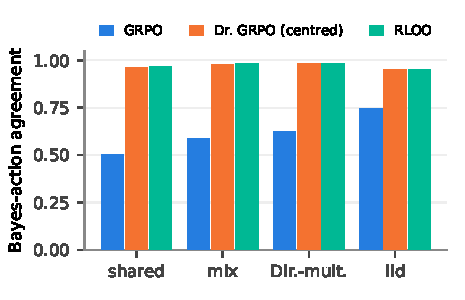
\includegraphics[width=\columnwidth]{figures_v4/fig_th1_laws.pdf}
\caption{Test~1: how often each estimator learns the value-optimal decision, by group law (731 problems, 10 seeds
each). Averaging-only estimators are unaffected by the law; GRPO is worst with shared worlds and still far off with
independent ones. Source: \path{results/theory/th1_heldout_summary.json}.}\label{fig:th1}
\end{figure}

\section{Test 2: a trained language agent}\label{sec:llm}
\paragraph{The agent and its tasks.} The policy is Tiny Aya Global, a 3.35B Cohere model
\citep{salamanca2026tinyayabridgingscale}. It works in ProcureSim, our simulated procurement system: it places supplier
orders, records receipts, pays and posts journal entries through tools, and each task carries one hidden fault plan
(60\% of tasks are clean). A deterministic verifier reads the final database and scores verified safe completion (VSC):
1 if every step really happened, with no duplicate payment, and the agent's report is true; 0 otherwise. The reward is
VSC minus $c=0.05$ per read. Training starts from a supervised warm start and runs GRPO through AgentTune's trainer
(4 tasks $\times$ 8 attempts per step, 200 steps). Every group shares its hidden world: we checked the code and all
800 logged groups of each run.

\paragraph{What carries over from the theory.} The stakes-cancel theorem applies directly. The exact vote does not,
because the agent's repair succeeds by chance; in that case the theory still predicts that GRPO responds to cost far
less than std-free does. So this test checks predictions derived from the theory, not the theorems themselves.

\paragraph{Design.} The registered comparison (\path{PREREGISTRATION_AD_C1.md}, called AD-C1 in the repository) trained
each method five times and scored VSC on 300 unseen tasks (121 faulted). Eight predictions were frozen in writing before
any result (\path{docs/research/AD_C1_THEORY_PREDICTION.md}). The test was an exact permutation test with a Holm
correction across four comparisons.

\paragraph{Results.} Standard GRPO never learned to check: all five runs read 0 times per episode and scored 0.687,
exactly the warm start. Std-free runs read 0.93 to 2.02 times per episode and scored 0.807 on average, $+0.120$ over
GRPO (95\% interval [0.088, 0.153] as registered; [0.075, 0.167] when runs are also resampled; Holm $p=0.016$; better
in all five pairs). The whole gain is on faulted tasks; on clean tasks both score 1.000. Seven of the eight frozen
predictions held; the eighth, about cost, needs a second cost, which Test~3 supplies.

\begin{figure}[t]\centering
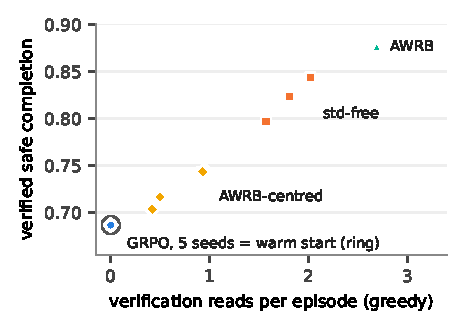
\includegraphics[width=\columnwidth]{figures_v4/fig_c1_seeds.pdf}
\caption{Test~2, one point per training run (300 unseen tasks). All five GRPO runs sit on the warm start (ring).
AWRB is an alternative return that averages over worlds the agent cannot tell apart. Source:
\path{results/ad/conf_summaries/}.}\label{fig:c1}
\end{figure}

\paragraph{What this result does and does not show.} Because all five GRPO runs ended at the same place as the warm
start, they are not five independent outcomes, and $p=0.016$ is simply the smallest value this test can produce. The
result shows that standard GRPO did not learn to check in this setup while std-free did; it is not evidence that GRPO
itself improved checking. One extra check, made after the registered analysis, separates ``GRPO did nothing'' from
``GRPO pushed checking down'': when actions are sampled, the warm start reads 0.189 times per episode, every GRPO run
0.000 to 0.001, and std-free 1.051. GRPO moved the agent away from checking, as the vote predicts.

\paragraph{More checking is not the goal.} One alternative return (AWRB, which averages the reward over worlds the
agent cannot distinguish) scores highest, $+0.192$ over GRPO, but reads 2.7 times per episode, far more than the faults
require, again as its vote predicts. Calibrated checking, not maximal checking, is what the value asks for.

\paragraph{Test 3: does the agent respond to the cost of checking?} The third registered test
(\path{PREREGISTRATION_AD_C2.md}, called AD-C2) retrained GRPO and std-free at a lower read cost, 0.01, and GRPO at
cost 0, one run each, and scored them with the cost-0.05 runs on a new sealed split of 300 tasks (120 faulted), five
episodes per task. The theory predicts that GRPO's vote only flips sign when reads become free (a clean world's
$\beta=-c$ is negative for every $c>0$), so GRPO should switch from never reading to reading only at $c=0$, while
std-free should read more as reads get cheaper. That is what happened (Table~\ref{tab:c2}): GRPO read 0.000 times per
episode at both 0.05 and 0.01, with identical completion (0.707), and 2.72 times at cost 0 (completion 0.883); std-free
read 1.81 times at 0.05 and 2.63 at 0.01 (+1.05 [+0.95, +1.15]), and beat GRPO at 0.01 by $+0.113$ [$+0.077$, $+0.152$].
All three primary and both secondary registered predictions held. Two caveats: each arm is a single run, and GRPO's
zero reads at 0.01 cannot by themselves tell ``ignores the cost'' from ``did not move''; the cost-0 run, where the same
recipe does learn to read, is what shows GRPO can move. A dated addendum before any result recorded a runner bug and
its one-line fix (\path{PREREGISTRATION_AD_C2_ADDENDUM2.md}); every model was still evaluated once.

\begin{table}[t]\centering\small
\resizebox{\columnwidth}{!}{%
\begin{tabular}{@{}lccccc@{}}\toprule
Arm & read cost & reads/ep & VSC & faulted VSC & false success\\\midrule
GRPO & 0.05 & 0.000 & 0.707 & 0.267 & 0.293\\
GRPO & 0.01 & 0.000 & 0.707 & 0.267 & 0.293\\
GRPO & 0 & 2.723 & 0.883 & 0.708 & 0.117\\
std-free & 0.05 & 1.810 & 0.803 & 0.508 & 0.197\\
std-free & 0.01 & 2.630 & 0.883 & 0.708 & 0.117\\\bottomrule
\end{tabular}}
\caption{Test 3 on the sealed split (300 tasks, 120 faulted; greedy decoding; one training run per arm). Source:
\path{results/ad/c2/c2_summary.json}.}\label{tab:c2}
\end{table}

In a related setting where reads are free, removing the standard
deviation did not help (0.813 against 0.819), which fits the theory: with free reads the worlds do not differ in
cost, so there is nothing for the vote to lose.

\section{Toolkits, models, data and metrics}\label{sec:kits}
\paragraph{Hackathon toolkits.} \textbf{AgentTune} \citep{lyngkhoi2026agenttuneunifiedtraininglifecycle} trains every
GRPO policy (its \texttt{TrlAgenticGrpo} trainer) and provides the tool-call parser and prompt used in training and
evaluation. \textbf{CuratorKIT} \citep{bhattacharjee2026curatorkitdatacuration} deduplicated the supervised recovery
demonstrations before the warm start (exact and MinHash; 0 of 554 removed). \textbf{AuditKIT}
\citep{arora2026auditkitunifiedevaluationspine} scored episodes with LLM judges as a secondary check; the database
verifier is always the primary truth. They connect in one line: CuratorKIT cleans the demonstrations, the warm start
learns from them, AgentTune runs GRPO on top, the verifier scores, and AuditKIT cross-checks. CircuitKIT was tried
and did not run; AlignTune and SafeTune were not used.

\paragraph{Models and licences.} Policy: \texttt{CohereLabs/tiny-aya-global} (3.35B, bf16, LoRA adapters,
CC-BY-NC-4.0). Aya Expanse 8B and 32B \citep{dang2024ayaexpansecombiningresearch} appear only as untrained comparison
agents and as a judge. No teacher model is distilled.

\paragraph{Data and splits.} All tasks are synthetic purchase orders generated in ProcureSim, in English. The agent
study trains on one split and evaluates on 300 unseen tasks; the cost test uses a new sealed split of 300 tasks, and a
script asserts that no task appears in two splits. The analytical test's 731 problems were frozen by hash before use.

\paragraph{Metrics.} Verified safe completion (higher is better), false success (claimed done but not done; lower is
better), reads per episode (should match the value of checking), and tool-call validity. Table~\ref{tab:track3} in
the appendix gives the Track~3 set per subset, with timing.

\section{Related work}\label{sec:related}
Dr.~GRPO \citep{liu2025drgrpo} removes the standard deviation to fix a bias toward easy prompts;
\citet{bay2026grpodrgrpodapo} relate GRPO, Dr.~GRPO and DAPO through the group standard deviation for right-or-wrong
rewards; \citet{fontana-etal-2026-hidden} show that the AdamW optimiser ignores a global rescaling of rewards. Our
invariance is different: it is per hidden world and comes from the group, not the optimiser. \citet{sakib2026luck}
pair rollouts on shared tool-fault schedules, which creates exactly our group structure, but study variance rather
than what the objective learns. Calibrate-Then-Act \citep{ding2026calibratethenactcostawareexplorationllm} prices
exploration and reports GRPO collapsing to one policy across costs, without stating how groups were formed. Work on
duplicates and silent tool failure \citep{li2026doesexactlyoncelivemodel,zhu2026evidenceguidedrecoveryaiagents,kaynar2026toolsfailagentsfabricate}
studies evaluation and inference; we study the training estimator. Appendix~\ref{app4:lit} compares them in detail.

\section{What to do about it}\label{sec:disc}
When the attempts in a group share a hidden world and the task has a costly information action, do not divide by the
group's standard deviation: subtract the mean only (Dr.~GRPO, RLOO), or use a scale that does not depend on the
group's hidden world. Shuffling worlds across attempts is not enough (Corollary~\ref{cor:homog}). More broadly, in agent
RL a group is not just a prompt; it can be a prompt plus a hidden world, and estimators should be analysed, and
training logs recorded, with that in mind.

\section*{Limitations}
The exact results cover one decision; for multi-step workflows the stakes-cancel theorem still holds but gives no
numbers. The language-agent evidence is one model family and one simulator, the GRPO arm of Test~2 did not move, and
the cost test has one run per arm and one group law. The cost re-scoring of training logs is
counterfactual, and the free-read explanation was made after the result. Reads are counted whether or not they were
informative. No human-labelled evaluation exists. The novelty is incremental over known z-score invariances
\citep{wang2026darkroom}: what is new is treating the hidden world as part of the group and working out its exact
consequences for a costly decision.

\section*{Ethics statement}
All tasks are synthetic and no real system is touched. The mechanism can make agents skip checks whose failures are
rare but costly; we recommend scales that do not depend on the hidden world, and deterministic verification of writes.

\section*{Acknowledgements and use of AI}
Lexsi Labs for the hackathon, its toolkits and HF credits; BITS Pilani HPC (sharanga) for GPU time; Cohere Labs for
Tiny Aya and Aya Expanse. Claude (Anthropic) was used to help write code and to help with writing.

\bibliography{refs_v4}
\bibliographystyle{acl_natbib}

\appendix
\section{Submission details (hackathon template)}\label{app4:submission}
{\small
\begin{description}\setlength{\itemsep}{1pt}
\item[Track and problem.] Track 3 (agentic fine-tuning), problem statement 9 (Measure $\rightarrow$ Understand
$\rightarrow$ Fix).
\item[One-line claim.] When the rollouts of a GRPO group share a hidden environment state, group-std normalisation
makes a costly check follow a vote of state-wise signs instead of its value; removing the std restores reading in a
3.35B Cohere tool agent.
\item[Before $\rightarrow$ after, same model.] Tiny Aya Global warm start 0.687 $\rightarrow$ std-free GRPO 0.807
verified safe completion (mean of 5 seeds; 300 unseen tasks), while standard GRPO from the same warm start stays at
0.687 in all 5 seeds (\S\ref{sec:llm}, Table~\ref{tab:track3}).
\item[Base model and method.] \texttt{CohereLabs/tiny-aya-global} (3.35B, CC-BY-NC-4.0), LoRA SFT warm start, then
GRPO through AgentTune's \texttt{TrlAgenticGrpo}, with and without the group std, read cost $c=0.05$.
\item[Real use case.] Agents that write to payment, order or deployment systems can read the record back before
reporting success; whether that check is learned depends on how training scales rewards inside a group.
\item[Hackathon kits.] AgentTune trains every GRPO policy and supplies the parser and prompt used in rollouts and
evaluation. AuditKIT gave the Stage~1 judge audit and secondary scores of the practical study's episodes. CuratorKIT
deduplicated the recovery demonstrations before SFT (0 removed). CircuitKIT was tried and did not run; AlignTune and
SafeTune were not used.
\item[Data and splits.] TH1: an analytical testbed with a held-out split frozen by hash
(\path{scripts/theory/freeze_th1.py}). Language agent: \texttt{cw\_train}, \texttt{cw\_dev}, \texttt{cw\_conf} (300
tasks, 121 faulted) and the sealed \texttt{cw\_c2} (300 tasks, 120 faulted); \path{scripts/ad/c2_split.py} asserts
that no task is shared across splits. Everything is generated in ProcureSim, an in-memory simulator; no real system is
touched.
\item[Metrics.] Verified safe completion (VSC: the final database meets every postcondition with no invariant
violation or duplicate, and the agent's report matches the expected status; \path{actionproof/env/verifier.py}), false success, reads per episode, tool-call validity; Table~\ref{tab:track3} gives the Track~3
set per subset.
\item[Declaration of work done outside the hackathon.] No part of this work predates 1 November 2026 (confirmed by the
author). Stage~1 (1--15 Nov): SupportSim and reward studies. Stage~2 (20--28 Nov): ProcureSim, the TXN benchmark and
the trained agents. The theory, TH1 (registered 24 Nov), AD-C1 (registered 23 Nov) and AD-C2 (registered 28 Nov) were
all done in the final round. The kits are the hackathon's own repositories at the stated revisions.
\item[With more credits.] The planned factorial: 2 estimators $\times$ 3 costs $\times$ 2 group laws (shared and
iid) $\times$ 5 seeds, plus a second model family. The theory predicts that GRPO's read rate stays flat in cost under
the shared law and responds to cost under the iid law, and that std-free tracks cost under both. These are
predictions, not results.
\item[Compute.] Training and evaluation ran on the BITS Pilani sharanga cluster (one H100 per run; each AD-C2 training
run was budgeted 150 minutes). TH1 ran on CPU (Appendix~\ref{app3:compute}).
\item[Use of AI.] Claude (Anthropic) wrote about 95\% of the code and drafted about 90\% of the text (author's
estimate). The research direction, the approval of every registration before its run, and the review of every claim
were the author's. Language-model judges are instruments and never replace the database verifier.
\item[Artefacts and running it.] Code: \url{https://github.com/atharvgaur1845/actionproof-v2} (branch
\texttt{submission-candidate}); live Space \texttt{atharvgaur18/actionproof-live}; traces
\texttt{atharvgaur18/actionproof-traces}. Commands: \texttt{pytest tests/theory};
\texttt{python scripts/s2\_numcheck.py}; \texttt{python scripts/ad/freeze\_c2.py --check};
\texttt{python scripts/ad/c1\_stats.py}; \texttt{python scripts/paper/v4\_figures.py};
\texttt{python scripts/paper/v4\_track3\_table.py}.
\end{description}}


% Appendix for main_v3.tex (research/latent-state-theory). Sources: docs/theory/*, docs/research/*, docs/judges/*.
\section{Implementation facts the theory relies on}\label{app3:impl}
\begin{itemize}
\item \textbf{Group key.} \texttt{actionproof/ad/pools.py} draws one fault plan per task and \texttt{make\_env\_cw}
applies it to every rollout. TRL~1.7.1 groups the $G{=}8$ completions of each prompt, and prompts are unique per task.
All 800 logged groups of every training run share one plan.
\item \textbf{Determinism.} The only environment randomness is id generation, which is hashed. Given the task and the
action sequence the return is deterministic, so within-group variation is policy sampling.
\item \textbf{Advantage.} \texttt{scale\_rewards="group"}: $(R-\bar R)/(\hat\sigma+10^{-4})$ with Bessel std;
\texttt{"none"} centres only.
\item \textbf{Loss.} The default \texttt{loss\_type="dapo"} normalises by the active tokens of the accumulated batch.
\texttt{num\_iterations=1} gives importance ratio 1, so clipping is inactive. KL $\beta=0.02$. Our ``Dr.~GRPO'' arm is
therefore Dr.~GRPO's advantage with DAPO aggregation; it differs from Dr.~GRPO's constant normaliser by one positive
scalar per step.
\end{itemize}

\section{Statements and proofs}\label{app3:proofs}
Notation as in \S\ref{sec:theory}. Assumptions:
These are the three assumptions of \S\ref{sec:setup}, numbered: \textbf{A1} (aliasing) the decision is aliased ($r\perp z$ given $h$);
\textbf{A2} (independence) rollouts are conditionally independent given the states;
\textbf{A3} (exchangeability) the group law is exchangeable with marginal $w$.

\paragraph{Proposition 1 (Bernstein form).} For a centred estimator ($\sum_iA_i=0$),
$\sum_iA_i(r_i-\pi)=\sum_{i:r_i=1}A_i$. Given the reader set $S$ with $|S|=k$, A1 and A3 make the law of
$(z,o,R)$ independent of $\pi$. It depends on $S$ only through $k$. Hence
$U(\pi)=\sum_kC(G,k)\pi^k(1-\pi)^{G-k}b_k$ with $b_k$ free of $\pi$ and $b_0=b_G=0$. Writing $t=\pi/(1-\pi)$,
$U=(1-\pi)^G\sum_kC(G,k)b_kt^k$, so by Descartes' rule the number of interior zeros is at most the number of sign
changes of $(b_1,\dots,b_{G-1})$. $\square$

\paragraph{Proposition 2 (centred estimators ignore the group law).}
$\sum_{S}d_i=(1-\tfrac kG)\sum_SR_i-\tfrac kG\sum_{\bar S}R_j$. By A1 and A3 each reader's state has marginal $w$, so
$\mathbb E[R_i\mid i\in S]=\mu_1$, and likewise $\mu_0$ for skippers. Hence $b_k=\tfrac{k(G-k)}G\Delta Q$. Summing
with $\mathbb E[k(G-k)]=G(G-1)\pi(1-\pi)$ gives $(G-1)\pi(1-\pi)\Delta Q$. For general trajectories, the cross terms
$\mathbb E[R_j\nabla\log\pi(\tau_i)]$ vanish because $\mathbb E[\nabla\log\pi(\tau_i)\mid z_{1:G}]=0$ under A2.
$\square$

\paragraph{Theorem 1 (per-state scale invariance).} Under the shared law every $R_i$ in a group comes from one state.
Since $\big((\lambda R_i+\kappa)-(\lambda\bar R+\kappa)\big)/(\lambda\hat\sigma)=(R_i-\bar R)/\hat\sigma$, the update
conditional on $z$ is unchanged. The unconditional update is the $w$-mixture of these. With $\epsilon>0$ the factor
$\lambda\hat\sigma/(\lambda\hat\sigma+\epsilon)$ remains. $\square$

\paragraph{Corollary 1 (vote).} If $R=\alpha_z+\beta_zr$ then $d_i=\beta_z(r_i-\bar r)$ and
$\hat\sigma_R=|\beta_z|\hat\sigma_r$, so the group's update is $\sgn(\beta_z)(G-1)\hat\sigma_r$. Taking the
expectation over $k$ and then over $z$ gives $(G-1)m_G(\pi)\mathcal V$. $\square$

\paragraph{Scope of $p\,s>1/2$.} With repairability in the state, the states are clean $(1-p)$, repairable $(ps)$
and unrepairable $(p(1-s))$, with $\beta=-c,\;V+L-c,\;-c$. So $\mathcal V=2ps-1$ whenever $0<c<V+L$.
Table~\ref{tab:thr3} gives exact thresholds when repair is rollout noise instead.

\begin{table}[h]\centering\small
\resizebox{\columnwidth}{!}{%
\begin{tabular}{llcccc}\toprule
$s$&$c$&$1/(2s)$&GRPO, $s$ in state&GRPO, $s$ as noise&Dr.~GRPO\\\midrule
1.0&0.01/0.05/0.2&0.5&0.495/0.499/0.500&same&$c$\\
0.6&0.01/0.05/0.2&0.833&0.825/0.832/0.833&0.654/0.667/0.706&$c/s$\\
0.3&any&1.67&never&never&$c/s$\\\bottomrule
\end{tabular}}
\caption{Smallest fault rate at which the expected update at $\pi=0.3$, $G=8$ is positive
(\path{results/theory/scan.json}).}\label{tab:thr3}
\end{table}

\paragraph{Corollary 2 (endogenous homogeneity).} With $G-1$ readers at a common return $R^\ast$ and one skipper at
$\alpha$: $d_{\rm skip}=(G-1)(\alpha-R^\ast)/G$, each reader has $d=-(\alpha-R^\ast)/G$, and
$\hat\sigma=|\alpha-R^\ast|/\sqrt G$. So $\sum_{\rm readers}A=(G-1)\sgn(\beta_{z_{\rm skip}})/\sqrt G$. The skipper's
state has marginal $w$ under every exchangeable law (A1, A3). $\square$

\paragraph{Proposition 3 (critical correlation).} For the mixture,
$b_1(\rho)=\rho b_1^{\rm sh}+(1-\rho)b_1^{\rm iid}$ and $b_1^{\rm sh}=(G-1)\mathcal V/\sqrt G$, so never-verify is
stable iff $\rho>\rho^\ast=b_1^{\rm iid}/(b_1^{\rm iid}-b_1^{\rm sh})$.

\paragraph{Propositions 4--6 (other estimators).}
\begin{itemize}
\item \emph{AWRB}: replacing $R$ by $\mathbb E[R\mid$ own observations$]$ gives every state $\beta=p(V+L)-c$ when
$s=d=1$ and the cost is state-independent. The vote is then $\sgn\Delta Q$. Otherwise the clean state's $\beta$
ignores $s$, which yields over-verification.
\item \emph{Per-component normalisation} of $(U,-cr)$: the cost component contributes $-(G-1)\hat\sigma_r$ in every
non-degenerate group; the utility component contributes 0 in the clean state and $+(G-1)\hat\sigma_r$ in a
repairable fault. So $U\le0$.
\item \emph{Zero-variance filtering} divides the update by $P(\text{non-degenerate})$.
\end{itemize}

\section{Counterexamples}\label{app3:counter}
Twenty-five perturbations, classified as (1) invalidates, (2) narrows, (3) coefficient only, or (4) irrelevant to the
implementation, are listed in \path{docs/theory/COUNTEREXAMPLES.md}. None is of class (1). The substantive class (2)
cases:
\begin{itemize}
\item severity, and rare catastrophic faults: GRPO's update is unchanged when the rare state's stakes are multiplied
by 1000;
\item state-dependent costs, which also break AWRB;
\item stochastic repair or detection as rollout noise, where the vote form must not be quoted;
\item exogenous within-state noise, which restores cost sensitivity: GRPO reaches the Bayes action at $q_0=0.3$;
\item independent states, which leave $\Theta(1/G)$ regret;
\item per-component normalisation, which never verifies.
\end{itemize}

\section{Test 1 (TH1): held-out analytical testbed}\label{app3:th1}
\textbf{Registration:} \path{PREREGISTRATION_TH1.md}, frozen before any held-out output
(\path{results/th1_hashes.json}). The design is in \S\ref{sec:th1}. Full criteria and descriptive results are in
\path{results/theory/th1_heldout_summary.json} and \path{docs/research/TESTBED_RESULTS.md}. Per-seed values are in
the shard files.

\section{Language-agent mechanism diagnostics}\label{app3:mech}
\path{docs/research/MECHANISM_DIAGNOSTICS.md} gives, per training run (18 runs), the following:
\begin{itemize}
\item read share by window;
\item early vote and $\Delta Q$ with bootstrap intervals;
\item last-window $\Delta Q$;
\item the variance source of clean groups;
\item the counterfactual cost sweep.
\end{itemize}

\section{Test 2 (AD-C1): the language-agent comparison}\label{app3:c1}
\textbf{Registration:} \path{PREREGISTRATION_AD_C1.md} with addendum~1 and notes~2--3, unchanged. The theory's
predictions T1--T8 (the eight frozen predictions of \S\ref{sec:llm}) were frozen before any confirmatory output in \path{docs/research/AD_C1_THEORY_PREDICTION.md}.
Result: \path{results/ad/c1_summary.json} (Slurm 469851). The per-seed table and the T1--T8 comparison are in
\path{docs/research/AD_C1_ANALYSIS.md}: T1--T7 are met and T8 is untestable.

\section{Judges}\label{app3:judge}
J2 (\path{PREREGISTRATION_J2.md}, Slurm 467652, \$2.816) is reported in \path{docs/judges/J2_FINAL_REPORT.md}, with
tables generated from \path{results/j2/j2_summary.json}.
\begin{itemize}
\item \textbf{Licences}, checked on the specific checkpoints' Hub cards:
\begin{itemize}
\item google/gemma-4-31B-it: Apache~2.0; the card links the Apache-2.0 text; no LICENSE file in the repository;
\item CohereLabs/aya-expanse-32b: CC-BY-NC-4.0 plus Cohere's Acceptable Use Policy;
\item Qwen3-235B-A22B-Instruct-2507 and gpt-oss-120b: apache-2.0;
\item DeepSeek-V3.2: MIT (Hub metadata).
\end{itemize}
\item \textbf{Human labels:} none exist; this is a model-versus-verifier study only.
\end{itemize}

\section{Compute and budget}\label{app3:compute}
\begin{itemize}
\item All theory and testbed computation ran on CPU Slurm jobs (compute partition, own working copy). The analytical
scan took 65\,s; each TH1 shard took a few minutes on 8 cores.
\item No GPU job was registered or run in this phase.
\item Judge spend: J1 \$3.20 and J2 \$2.82 (token-priced estimates, \path{docs/stage2/HF_CREDITS.md}).
\end{itemize}

\section{Reproduction}\label{app3:repro}
{\footnotesize\begin{verbatim}
pytest tests/theory
python scripts/theory/scan.py
python scripts/theory/freeze_th1.py \
  --check
sbatch --array=0-11 --export=\
  ALL,SPLIT=heldout,NSH=12 \
  slurm/theory/th1_array.sh
python scripts/theory/th1_analyze.py \
  --split heldout
python scripts/theory/llm_mechanism.py \
  --rollouts <dir>
\end{verbatim}}

\section{Test 1: all ten estimators}\label{app4:est}
\begin{table*}[t]\centering\small
\resizebox{0.9\textwidth}{!}{%
\begin{tabular}{@{}lccccc@{}}\toprule
Estimator & Bayes agreement & mean regret & median regret & regret shared & regret iid\\\midrule
GRPO & 0.596 & 0.610 & 0.065 & 0.676 & 0.364\\
GRPO + zero-var.\ filter (DAPO) & 0.596 & 0.601 & 0.034 & 0.668 & 0.356\\
GRPO + KL & 0.595 & 0.610 & 0.073 & 0.676 & 0.360\\
Dr.~GRPO (centred) & 0.970 & 0.011 & 0.009 & 0.012 & 0.012\\
RLOO & 0.974 & 0.008 & 0.007 & 0.008 & 0.008\\
REINFORCE (EMA baseline) & 0.975 & 0.008 & 0.007 & 0.009 & 0.008\\
batch std & 0.949 & 0.043 & 0.009 & 0.045 & 0.029\\
PPO (4 clipped epochs) & 0.947 & 0.040 & 0.004 & 0.063 & 0.015\\
AWRB (obs.-measurable return) & 0.903 & 0.031 & 0.004 & 0.056 & 0.015\\
per-component norm.\ (GDPO-style) & 0.222 & 1.914 & 0.509 & 1.537 & 2.197\\\bottomrule
\end{tabular}}
\caption{TH1 held-out, 731 cells, 10 seeds per cell, synthetic trainer (not language-model runs)
(\path{results/theory/th1_heldout_summary.json}, \texttt{descriptive}). Mean regret is dominated by high-severity cells.}\label{tab:est}
\end{table*}

\section{Test 2, run by run}\label{app4:seeds}
\begin{table*}[t]\centering\small
\resizebox{\textwidth}{!}{%
\begin{tabular}{@{}lccccc@{}}\toprule
Arm ($c=0.05$) & seed & VSC & reads/ep & false success & faulted VSC\\\midrule
warm start & -- & 0.687 & 0.000 & 0.313 & --\\
GRPO & 0--4 & 0.687 (all) & 0.000 (all) & 0.313 & 0.223\\
std-free & 0/1/2/3/4 & .827/.797/.823/.743/.843 & 1.80/1.57/1.80/0.93/2.02 & .173/.200/.173/.253/.157 & .570/.496/.562/.364/.612\\
AWRB & 0--4 & 0.877--0.880 & 2.69--2.70 & 0.120 & 0.694--0.702\\
AWRB-centred & 0/1/2/3/4 & .743/.743/.703/.687/.717 & .96/.93/.42/.00/.50 & .253/.253/.293/.313/.283 & --\\\bottomrule
\end{tabular}}
\caption{AD-C1 greedy evaluations on cw\_conf (300 tasks, 121 faulted) (\path{results/ad/conf_summaries/},
\path{docs/research/AD_C1_ANALYSIS.md}). AD-C2 per-arm results are not part of this version (runs incomplete when it was frozen).}\label{tab:seeds}
\end{table*}

\section{The practical ActionProof study (context)}\label{app4:practical}
The simulator used here comes from a larger practical study, reported separately
(\path{paper/actionproof_main.pdf}). Its registered results, with their limits:
\begin{itemize}
\item \textbf{P1}, the registered recovery-training comparison (450 frozen tasks, 3 seeds): recovery supervised fine-tuning (SFT) reaches 0.772 and recovery SFT then GRPO 0.819 sampled VSC
against 0.513 for the reference arm A, itself a trained agent (recovery-start GRPO); the untrained Tiny Aya Global
base scores 0.01 on the same test (\path{results/p5/p5_summary.json}). The arms are not nested checkpoints, so the
difference is not GRPO's alone.
\item \textbf{TXN v1}, the transaction benchmark (440 locked counterfactual tasks): trusting the reply falsely completes 0.864 of tasks; the
trained agent 0.121; a hand-written reconciliation script beats every learned agent (verified task completion, VTC, 0.864; no false completion).
A post-hoc review found construct limits: a read-free same-key double send reaches 308 of 440, and the duplicate
metric counts injected duplicates.
\item \textbf{P4 and P5}, the transfer studies: randomised demonstrations improve the SFT warm start on renamed tools (+0.604) and an unseen
workflow (+0.574), not shown after GRPO; the recipe lifts four more Cohere bases (one SFT seed each).
\item \textbf{SEL1}, the selective hand-off study: supervised hand-off after repeated outage errors (0.972 against 0.002); where hand-off is the only
safe action it helps in 164 of 432 episodes.
\item \textbf{RG1 and RG2}, the Recovery Gate studies: a rules-based runtime gate takes false completion from 0.112 to 0.000 on a sealed split, by
construction (a consistent read is a perfect oracle in the simulator); most of its hand-off gain relabels honest
failures; the script still completes more. It is not a learned-policy contribution.
\end{itemize}

\begin{table*}[t]\centering\small
\begin{tabular}{lcccccccc}\toprule
Arm (seeds) & \multicolumn{3}{c}{Task success (VSC)} & False & Tool-call & Calls & Reads & Eval s \\
 & all & faulted & clean & success & validity & /ep & /ep & /300 tasks \\\midrule
Warm start (1) & 0.687 & 0.223 & 1.000 & 0.313 & 1.000 & 3.73 & 0.00 & 14 \\
GRPO (5) & 0.687 {\scriptsize [0.687, 0.687]} & 0.223 & 1.000 & 0.313 & 1.000 & 3.73 & 0.00 & 14 \\
Std-free (5) & 0.807 {\scriptsize [0.743, 0.843]} & 0.521 & 1.000 & 0.191 & 1.000 & 5.46 & 1.62 & 22 \\
AWRB (5) & 0.879 {\scriptsize [0.877, 0.880]} & 0.699 & 1.000 & 0.120 & 1.000 & 6.61 & 2.69 & 24 \\
AWRB-centred (5) & 0.719 {\scriptsize [0.687, 0.743]} & 0.302 & 1.000 & 0.279 & 1.000 & 4.31 & 0.56 & 16 \\
\bottomrule\end{tabular}
\caption{Track 3 metrics for the AD-C1 arms (descriptive; means over seeds, greedy decoding, 300 unseen \texttt{cw\_conf} tasks: 121 faulted, 179 clean; range over seeds in brackets). Eval seconds are wall time for the whole batched split on one GPU, not per-request latency. Batch-1 latency was measured on the same Tiny Aya Global base with a LoRA adapter (40 ProcureSim dev episodes): warm start 2.44\,s per episode (p95 3.05\,s), database-reward GRPO agent 3.82\,s (p95 4.68\,s), whose episodes include read-backs. Sources: \path{results/ad/track3_metrics.json}, \path{scripts/paper/v4_track3_table.py}.}\label{tab:track3}
\end{table*}

\section{Literature comparison: what was read}\label{app4:lit}
Full text (2026-11-28): \citet{fontana-etal-2026-hidden} (Props.~1--3: shared-prefix weighting; AdamW invariance to
global reward scale; momentum overshoot past the clip); \citet{bay2026grpodrgrpodapo} (Thm.~1: for binary rewards the
GRPO gradient is $\sigma(\bar s_+-\bar s_-)$ with $\sigma=\sqrt{k(G-k)}/G$; iid rollouts per prompt; no environment
state); \citet{sakib2026luck} (paired common-random-number schedules of tool faults and grader flips; variance
decompositions; no analysis of the std-normalised objective; no verification action); and
\citet{ding2026calibratethenactcostawareexplorationllm} (cost as a reward discount; GRPO ``collapse[s] to a static
test-first policy''; group construction not stated in the main text). Abstracts only: LIMBO, Evidence-Guided Recovery,
\citet{kaynar2026toolsfailagentsfabricate}.

\end{document}
